\chapter{Security in software development}
\label{ch:related}

Software security is a relatively new field.
The first books and academic classes on the topic appeared in 2001~\cite{mcgraw2004software}.
Despite that, many tools and practices have been developed over the past two decades that have greatly advanced this field.
In this chapter, I provide a broad overview of security practices and tools, discussed in order of their use in the \gls{sdlc}.
I also discuss a selection of specific tools in Appendix~\ref{app:battlecards}.
This appendix contains a number of battlecards in which I describe several tools that have caught my attention during this research.

\summarybox{
findings and conclusion
}

\section{Governance}
\label{sec:related-plan}

\subsection{Training}
Training has always played a critical role in software development, because standard computer science and engineering education often neglects software security.

Companies should first offer security awareness training to all employees involved in the software development life cycle.
Security awareness training does not necessarily need to be tailored to a specific audience.
Developers, \gls{qa} engineers, project managers, and operators can all partake in the same training.
A generic introductory course like this however is insufficient, the next step is to provide role-specific individual training.
As explained in this work, developers should be taught secure coding, and not follow training intended for security professionals or penetration testers.

In the ideal scenario, a company should also verify or provide training for vendors and contractors.
They should require annual refreshers for all employees and can host software security events to nurture a good security culture.

\subsection{Compliance and policy}
Software security is not only a problem of enablement.
Good enough training, tools, and processes exist today that can embed security in software development from the start.
Yet, we still see frequent reports in the media of bad software practices and vulnerabilities that easily could have been prevented.
The reality is that businesses often prioritize getting to market and getting new features out, over their obligations in terms of security.

\subsubsection{Privacy and trust}
The resulting security problems, however, do not only hurt the business, they also hurt the consumer.
When businesses are hacked, it is often private data of consumers that is leaked.
Recently, consumers have claimed control and rights over their personal data.
Legal frameworks have been built around data privacy, forcing businesses to consider data protection more seriously.

Most famously the \gls{gdpr}, a law on data protection and privacy, is enforced in the \gls{eu} since May 25, 2018~\cite{gdpr}.
It contains regulations that strengthen the individual's fundamental rights in the digital age and clarify rules for businesses storing or processing personal data of individuals in the \gls{eu}.
This law forces businesses to consider security more seriously, as it is estimated that at least 25\% of software vulnerabilities have \gls{gdpr} implications~\cite{gdprhackerone}.
Non-compliance with the general data processing principles in this law can result in significant fines, for example in June 2021, Amazon was fined €746 million\footnote{\url{https://www.enforcementtracker.com/ETid-778}}.
Two years after the implementation of the \gls{gdpr}, the \gls{ec} found that individuals' knowledge about data privacy has increased, and as a result privacy has become a competitive quality for companies which consumers are taking into account in their decision-making~\cite{gdprfra}.

Security is no longer just a necessary cost during development, but businesses are able to see a more direct \gls{roi} for high quality software security.
Businesses put more effort into the appearance of having trustworthy data protections in place, a process called trust management~\cite{cassandra2021analysis, ashraf2020role}.
In this discipline, consumer trust is the end-goal and good security practices are a mean to this goal.
To convince consumers and buyers of software to trust a product, businesses can acquire a seal of approval from a third party to prove they adhere to certain standards.
One such widely known certification is the \gls{iso}/\gls{iec} 27000-series, or ISO27K for short.
The series provides best practice recommendations on information security management, covering privacy, confidentiality, and other cybersecurity issues~\cite{iso27k}.
Other regimens that companies often aim to comply with are \gls{pci} and \gls{hipaa}.
To add transparency, businesses can also provide a \gls{sbom}, that lists all components used in their software~\cite{sbomntia}.
Such an \gls{sbom} is most easily produced using build tools as explained in Section~\ref{sec:related-build}.

In the \gls{us} Biden \gls{eo} on Improving the Nation's Cybersecurity issued May 12, 2021 the \gls{nist} was ordered to publish guidelines regarding practices that enhance the security of the software supply chain.
Besides providing the purchaser with such an \gls{sbom}, there are numerous other standards and procedures listed regarding trust, multi-factor authentication, encryption, and use of automated security tools.
In this \gls{eo}, \gls{nist} is directed to solicit input from the private sector and academia to develop standards, tools, and best practices.
Among the more than 150 position papers, dr. Matias Madou, dr. Brian Chess, and I have also submitted two.
One position paper advises the creation of a certification framework for education in secure development practices.
The second promotes the use of the paved path methodology.
Time will tell if this \gls{eo} makes a similarly big impact as the \gls{gdpr}.

Besides the \gls{gdpr} and the \gls{us} \gls{eo}, there are of course similar laws in other parts of the world such as the Data Protection Act in the United Kingdom, the Privacy Act in Canada, and the Personal Data Protection Bill in India.

\subsubsection{Law enforcement access}
Unfortunately, no discussion on laws and data privacy would be complete without mentioning laws on the collection and storage of electronic communication and their access by authorities.
Many of these laws contain requirements that force operators of end-to-end encrypted systems to undermine this encryption, so that law enforcement can be provided access to user communications.
One such example is the draft considered by the Belgian government at the end of September 2021\footnote{\url{https://ibpt.be/index.php/operateurs/publication/annexe-1-dispositif}}.
Under this law, operators would have to be able to ``turn off" encryption for specific users, essentially creating so-called backdoor access.
The consensus among cybersecruity experts is that there is no way to provide third party access like this to end-to-end encrypted communications, without also creating encryption backdoors and vulnerabilities that can be exploited by malicious third parties~\cite{bliss1996effective}.
Creating a backdoor like this, undermines the whole security of the system and puts its users at risk~\cite{encryptionmyths}.

In other countries where similar legislations have passed, such as Australia, research has shown that this has discouraged companies from offering new end-to-end encrypted products~\cite{barker2021economic}.
It is safe to say that policy makers and governments can have a big influence on the security of software products, for better or for worse.
\section{Develop}

Developer toolkits evolve over time, and many new technologies and frameworks exist to help developers produce code more efficiently, and more securely.
As explained in Section~\ref{sec:traditionalsecurity}, security tools are handed to the developer as well because a shift left movement is ongoing to try and identify possible security problems as early as possible in the \gls{sdlc}.
These tools, however, still use a reactive testing-based approach and can usually only identify security problems once sufficient code has been developed.
These tools will be discussed in the section on testing, Section~\ref{sec:related-test}.
In this section, I discuss tools and practices that help a developer securely produce code from the start.

\subsection{Lint}
Linter tools are designed to allow the developer to concentrate solely on the algorithms, data structures, and correctness of the program, and only later, with the aid of lint, address non-functional aspects of the code.
They mostly focus on syntax and styleguide checking but some tools are advanced enough to check for certain bugs as well.
Depending on their targets, linters perform their analyses with string-matching or reduced versions of \glspl{ast} without symbol information.
The more advanced lint tools perform similar analyses to Sensei, making use of the entire \gls{ast}.
Lint tools are useful and commonly used, but they are not often deployed for security purposes.
Some examples of lint tools are Error Prone\footnote{\url{http://errorprone.info/}}, Checkstyle\footnote{\url{http://checkstyle.sourceforge.net/}}, PMD\footnote{\url{https://pmd.github.io/}}, and SonarLint\footnote{\url{https://www.sonarlint.org/}} (Appendix~\ref{app:battlecards}, battlecard~\ref{bc:sonarlint}) by SonarSource.
Lint tools are also often included by default in \glspl{ide} such as AndroidStudio\footnote{\url{https://developer.android.com/studio/write/lint}} and IntelliJ IDEA\footnote{\url{https://www.jetbrains.com/help/idea/code-inspection.html}}.
Not many security rules are included in lint tools by default.
Out of the tools above, SonarLint supports the most, with 29 rules targeting vulnerabilities in Java\footnote{\url{https://rules.sonarsource.com/java/type/Vulnerability}}.
This is because lint tools require fast response times and scanning for vulnerabilities often takes longer-running analyses.
Many lint tools are open-source which means their rules can be customized to enforce secure coding guidelines, but none are designed for easy and fast customization of the rules.

\subsection{Security patterns}
Research has shown that adherence to secure coding guidelines leads to more secure code~\cite{lipfordimpact}.
It comes as no surprise that many efforts exist both in industry and in research to develop such guidelines.
In contrast with vulnerability lists, discussed in Section~\ref{sec:related-test}, these patterns provide proactive guidelines targeting developers.
Many of these guidelines can be used as a basis to create Sensei recipes, or rules for similar tools, provided they are specific enough.

Some provide sufficiently clear \gls{api}-level instructions that can directly be implemented as recipes in our plugin.
We have demonstrated this by creating a rule set from The Android Application Secure Design/Secure Coding Guidebook by the Japan Smartphone Security Association~\cite{jssec}.
Other notable examples are the guidelines designed to counter side-channel attacks, designed by Witteman~\cite{witteman2008secure}, and the Oracle Coding Standards\footnote{\url{https://wiki.sei.cmu.edu/confluence/display/java}}.
The Java code issues and transformations in these guidelines fall clearly within the capabilities of Sensei.

Other  guidelines are too generic and high level such as the work by Schumacher et al.~\cite{schumacher2013security}, or the \gls{owasp} Proactive Controls\footnote{\url{https://owasp.org/www-project-proactive-controls/}}.
In order to support these with Sensei or other tools, they need to be translated into concrete guidelines and customized for the used \glspl{api}.
For example, the \gls{owasp} Proactive Control number 5 instructs to validate all inputs.
To apply this proactive control in practice, security libraries have to be developed or selected to perform the input validations.

Some efforts have also been made to automatically generate rules from code changes such as Paletov et al.~\cite{paletov2018inferring}.
As mentioned in Section~\ref{sec:improvedrulecreation}, in the future we also want to develop such automatic recipe creation methods.

\subsection{Security Libraries and Frameworks}
Another solution to make developers adhere to coding guidelines, is by implementing them into frameworks or libraries.
An example is the \gls{owasp} \gls{esapi}, an open-source application security control library that provides clear replacement \glspl{api} for insecure \gls{jdk} implementations~\cite{ESAPI}.
As mentioned in this work, Sensei recipes have already been developed to support replacing banned methods with alternatives from the \gls{esapi} as a demonstration of library adoption recipes. 

Popular web application frameworks provide methods for sanitizing inputs and escaping outputs to prevent common vulnerabilities.
These frameworks are creating a paved path for developers to follow.
We have observed that these efforts result in useful code examples in the documentation of frameworks that are easy to understand for developers.
They also make for easy development of Sensei recipes to adhere to these guidelines.
However, the implementation details of these methods are sometimes lost to developers, and the results from this work show that this can sometimes lead to increased difficulty locating vulnerabilities.

Nonetheless, this evolution in frameworks has shown to be effective at preventing security problems as indicated by the position of injection flaws and \gls{xss} in the \gls{owasp} top 10.
Despite \gls{xss} attempts remaining common~\cite{trustwave}, the vulnerability has moved from third place in 2013, to seventh place in 2017.
In 2021 it is likely to merge with injection flaws, as shown in Figure~\ref{fig:newowasptop10} on page~\pageref{fig:newowasptop10}.
%At \glsc{scw}, we have observed the similarity between these two categories based on the Sensei recipes targeting both these categories.
After being the top category since 2013, injection flaws are likely to move down to the third position in the \gls{owasp} top 10 2021.




\todo[inline]{if time left}
github copilot
amazon guru
deepcode
\section{Build}
\label{sec:related-build}

There is an evolution in software development towards increasingly iterative and feedback-driven strategies.
Most noticeable is the Agile development model, formally introduced in 2001, where customer collaboration and responsiveness to change are key components~\cite{fowler2001agile}.
The highest priority in this model is to satisfy the customer through continuous delivery of valuable software, by welcoming changing requirements, even late in development.
Working software has to be delivered frequently, in a couple of weeks to a couple of months.
Product management and developers have to work closely together to set priorities and iteratively deliver minimal viable products and improvements.
In this process, individuals and interactions are prioritized over processes and tools, and working software is prioritized over comprehensive documentation.
The Scrum framework is frequently used to implement this type of development strategy~\cite{schwaber2004agile}.

Building on agile practices, \gls{devops} aims for complete end-to-end automation of not only software development, but also delivery.
In academic research, there is not yet a clear definition for \gls{devops}, but it is most often characterized by cross-functional teams and shared ownership~\cite{erich2017qualitative,ebert2016devops}.
Quality deliveries with short release cycles need a high degree of automation, and many tools have been developed to assist with this automation.

Build tools are used for compiling code, they often include so-called package or dependency managers to centralize project dependencies.
Some examples of build tools and package managers are Apache Ant\footnote{\url{https://ant.apache.org/}}, Maven\footnote{\url{https://maven.apache.org/}}, Gradle\footnote{\url{https://gradle.org/}},
Pip \footnote{\url{https://pypi.org/project/pip/}} and Yarn\footnote{\url{https://classic.yarnpkg.com/en/}}.

Managing dependencies centrally like this makes it easy to monitor and update to newer versions.
This also provides a centralized overview of all software components used to create a \gls{sbom} as explained in Section~\ref{sec:related-plan}.
Use of vulnerable and outdated components is a common vulnerability category, and part of the \gls{owasp} top 10.
Many \gls{sca} tools exist that scan build files and alert developers when the dependencies contain vulnerabilities.

% Battlecards
Some noteable tools are Snyk (battlecard~\ref{bc:snyk}), Dependabot (battlecard~\ref{bc:dependabot}) and GitLab Dependency Scanner (battlecard~\ref{bc:gitlab}).
These tools are typically integrated into the code repository and run regular scans.
Use of vulnerable components is a vulnerability that can be introduced \textit{after} initial development because dependencies are (supposed to be) updated frequently.
It makes sense to integrate this type of security tool in the code repository rather than development tools.
In the development tool, many developers would get notified of an outdated dependency at the same time, while likely few of them would be working on the build file.
This would either result in many \glspl{efp}, or in the same fix being applied by multiple developers.
Remediation for these vulnerabilities is often simply bumping the dependency to the newest version, and results from the Rasch model show that developers have no difficulty fixing this type of vulnerability.
Some \gls{sca} tools will calculate the minimal upgrade path so as not to risk any breaking changes in the code base.
As remediation guidance \gls{sca} tools often create automated pull requests that update dependencies to the newest version.
This process is intuitive and well integrated with existing developer workflows.

However, many challenges remain in this field, as in some programming languages over 70\% of vulnerabilities are in transitive dependencies~\cite{snyk2020}.
These can not be easily fixed since they are out of the control of the developer, if the direct dependencies are not updated, then they might need to be replaced.
With some package managers (such as Maven) it is also possible to exclude the transitive dependency and manually download the newest version, with the risk of runtime errors if there are any breaking changes.
Sometimes it can suffice to make sure methods containing vulnerabilities are not used, or they can be excluded or replaced with a so-called monkey-patch\footnote{\url{https://docs.plone.org/appendices/glossary.html\#term-Monkey-patch}}.
All these options require more initimate knowledge of the package manager or the dependencies being used.




\section{Test}
\label{sec:related-test}

Software security initially started as part of software testing~\cite{sharma2017}.
Today, still, most security practices are done in the testing phase.
Some part of software security will always be reactive.
Like all other parts of computer science, security keeps advancing, and we will always know more tomorrow than we know today.

So while many novel security tools and practices have been introduced and proven to be effective, new practices generally do not replace old ones.
Instead, they are added to the arsenal of weapons that is available for development and security teams.
In this section, I describe new tools and practices as well as some traditional ones, as I believe they will stay relevant, even if new tools and practices are being introduced.

\subsection{Penetration testing}
Penetration testing is the practice of breaking into running software by attacking it.
Sometimes, the penetration tester has access to the source code to speed up this process.
It is a common practice used by many companies and usually external experts are hired to perform these tests~\cite{cruzes2017security,bsimm11}.
Since the penetration tester needs access to the running software this can only be done very late in the \gls{sdlc}.
Already in the introduction, we addressed that relying on security experts does not scale well.
Furthermore, it does not integrate well in modern development strategies, where fast feedback cycles and frequent releases are key~\cite{securitytestingagile}.
Penetration testing does improve the security awareness of the developers, but does not cause any long-lasting change in development practices by itself~\cite{turpe2016penetration}.

\subsection{Code reviews}
To develop new features or fix bugs, a developer starts from a copy of the current codebase.
As other developers submit changed code, this copy gradually ceases to reflect the main (or master) version.
The longer development continues, the greater the risk of conflicts when merging work back into the main version.
A code review is a manual inspection of produced code that is performed when this work is merged back.
It is usually done by another developer than the original author but with that author present.
Code reviews also provide an educational aspect for the developer whose code is reviewed~\cite{futcher2008guidelines}.
The downside is that, similarly to penetration testing, it relies on internal or external experts and hence does not scale well.

\Gls{ci} tools are developed to merge the working copies of developers into a shared main version and automatically build and review code as frequently as possible.
A build server is usually set up for this purpose, that will build and test the code after every commit and report the results back to developers.
This testing is done with automated tools, such as static analysis tools.

\subsection{Static analysis}
Static analysis tools are well researched~\cite{li2017static,jovanovic2006pixy,livshits2005finding} and commonly used to detect vulnerabilities~\cite{cruzes2017security,bsimm9,bsimm11}.
Most tools can run automatically, and as a result are easily adapted in modern development strategies.
Static analysis tools vary from robust and time-consuming analyses such as Fortify~\cite{chess2004static} (battlecard~\ref{bc:fortify}) to light real-time analyses~\cite{brown2016build}.
In controlled experiments, static analysis tools proved to be more effective than penetration testing~\cite{Scandariato2013}.

\todo{whole list of tools that can be discussed}
Already mentioned in this work:
FindBugs
Fortify
Semgrep

As explained in this work, frequent testing is useful, but analyses of traditional security tools often run too long to be well-integrated in developer workflows.
These tools are often seen as a big inhibitor for the developer's productivity.
To mitigate this, a shift left movement is ongoing to apply them as early as possible in the \gls{sdlc}.

However, static analysis tools require sufficient code to be completed in order to detect vulnerabilities, and hence can usually not be used in a proactive manner.
By customizing the rules, some tools can be tailored to ignore context, which can speed up their analyses even if they were not designed with this in mind.
But even if local versions of the analyses perform well, they often do not provide fixes to resolve the discovered issues and hence do not enforce a paved path.
They can not be applied in a pro-active manner, like Sensei can.
An example of a tool that does provide fixes in the code review stage, is Tricorder~\cite{sadowski2015tricorder} (battlecard~\ref{bc:tricorder}), or its open source version Shipshape (battlecard~\ref{bc:shipshape}).
Research with this tool showed that most developers go back to their \gls{ide} rather than use the code review tool to resolve the issues~\cite{sadowski2015tricorder}.

\subsection{IDE-based}
Because developers prefer to remediate problems in their \gls{ide}, and as part of the shift left movement, many static analysis tools are now available as \gls{ide} plugins as well.
For some tools no effort has been made to adapt them to better suit the developer.
They still perform identical analyses to the original tool, either remotely or locally.
Some tools even prevent the developer from making changes to the code while the scan is in progress.
Examples of plugins like this are Semgrep, FindBugs/Spotbugs
\todo{examples: Semgrep, FindBugs/SpotBugs}

Performing the full scan, however, often takes too long and as a result these tools are not very usable.
In an attempt to be more developer-friendly, other tools provide lightweight versions of the analyses.
\todo{examples: Fortify Security Assistant}

In this case, the plugin is often not able to detect the complete set of vulnerabilities that the original tool is capable of.
The goal is to provide faster feedback loops to the developer, with the drawback that some of the vulnerabilities will go unnoticed.
But by detecting a portion of the vulnerabilities earlier in the \gls{sdlc}, they become easier and less expensive to fix.
All the other vulnerabilities are still caught when the fully capable tool is used in later phases of the \gls{sdlc}

\subsection{Rule customization}
For these tools to be most effective, their rules should be tailored specific to the organization's coding standards and target vulnerabilities relevant to the organization's history~\cite{bsimm9,bsimm11}.
As described in this work, this also prevents false positives and \glspl{efp}, thus improving usability for developers and ensuring continued use of the tool.

To customizes the rules, different approaches exist.
In this section, they will be demonstrated with a rule to detect the use of the deprecated cryptographic algorithm \gls{des} in Java.
The insecure line of code that needs to be marked is shown in Listing~\ref{lst:useDES}.

\begin{lstlisting}[language={Java},caption={Insecure use of a deprecated cryptographic algorithm},label={lst:useDES},abovecaptionskip=-0.0pt,xleftmargin=15pt]
Cipher.getInstance("DES");
\end{lstlisting}

\subsubsection{API}
The first method of rule customization is through use of an \gls{api}.
These tools require the rule-writer to write code that extends the functionality of tool so that it performs additional analyses.
The tool, or sometimes only the extension itself, then needs to be built into a new executable that can be used to analyse software products.
For Shipshape it is even required to expose this executable as a service using a docker image\footurl{https://github.com/google/shipshape}.

Creating detectors through an \gls{api} allows sufficient flexibility, but makes it more complex to develop and test custom rules.
SpotBugs (battlecard~\ref{bc:SpotBugs}) is an example of a tool that uses an \gls{api} for rule customization by creating so-called third party ``detectors"~\cite{spotbugsapi}.
These detectors have to be implemented and compiled into a SpotBugs plugin.
FindSecBugs~\cite{findsecbugs} is a popular security plugin for SpotBugs.
A detector to mark use of the \gls{des} algorithm is already implemented by the FindSecBugs plugin.
In Listing~\ref{lst:detectDES-findbugs}, a snippet of the class \texttt{DesUsageDetector} is shown that implements this detector.
This code is copied from the \texttt{find-sec-bugs} project on GitHub\footnote{\url{https://github.com/find-sec-bugs/find-sec-bugs}}.
The class extends the abstract class \texttt{CipherDetector} that is also implemented by the plugin, and hence not an \gls{api} provided by the original tool.
To create a detector for such a relatively simple example, multiple files and many lines of code are already needed that require sufficient knowledge of the \glspl{api}.
While the creation of additional detectors is not as convenient as creating recipes with Sensei, at least the distribution of detectors through a plugin is convenient for users of the tool.

\begin{lstlisting}[language={Java},caption={Rule customization of SpotBugs is done through java code using their API.},label={lst:detectDES-findbugs},abovecaptionskip=-0.0pt,xleftmargin=15pt]
public class DesUsageDetector extends CipherDetector {
    ...
    @Override
    int getCipherPriority(String cipher) {
        cipher = cipher.toLowerCase();
        if (cipher.equals("des") || cipher.startsWith("des/")) {
            return Priorities.NORMAL_PRIORITY;
        }
        return Priorities.IGNORE_PRIORITY;
    }
    ...
}
\end{lstlisting}

\subsubsection{Custom query language}
To make customisation of rules easier, some tools provide a custom query language that makes abstractions of their \gls{api}.
They still require the rule writer to write code, but they usually provide more specific syntax to make the development of rules much simpler.

Code Query Language (CodeQL) is an example of such a query language.
It is a free and open-source semantic code analysis engine that is created with the goal to query code as if it were data.
It borrows syntactic elements from data query languages such as \gls{sql} as well as elements from Java.
CodeQL is used by the popular analysis platform Semmle (battlecard~\ref{bc:semmle}).
A CodeQL query that detects use of \gls{des} is shown in Listing~\ref{lst:detectDES-semmle}.
This query is less complex and easier to write compared to using an actual \gls{api}.
CodeQL provides an online ``Query console" that makes development of these queries easier.
It provides syntax highlighting and auto-completion.
With this console it is also possible to test the queries on several demo projects.
The available projects do not necessarily contain the code a rule-writer is targeting, as was the case for the example rule.
None of the 7 available projects is using the \gls{des} encryption algorithm.

\begin{lstlisting}[language={sql},caption={CodeQL query used by Semmle to find use of insecure algorithm DES.},label={lst:detectDES-semmle},abovecaptionskip=-0.0pt,xleftmargin=15pt]
import java
from MethodAccess call, Method method
where
  call.getMethod() = method and
  method.hasName("getInstance") and
  method.getDeclaringType().hasQualifiedName("javax.crypto", "Cipher") and
  method.getParameter(0).toString().regexpMatch("DES.*")
select call
\end{lstlisting}

The query language CxQuery by Checkmarx uses regular Java syntax.
It provides abstractions to iteratively filter results based on certain properties of the code.
Some knowledge of the \gls{api} is required, but Checkmarx provides very clear and easy to understand documentation containing lots of examples.
The resulting query, shown in Listing~\ref{lst:detectDES-checkmarx}, is even shorter than the one for CodeQL and just as easy to understand.

\begin{lstlisting}[language={Java},caption={CxQuery query used by Checkmarx to find use of insecure algorithm DES.},label={lst:detectDES-checkmarx},abovecaptionskip=-0.0pt,xleftmargin=15pt]
result = All.FindByName("*getInstance*",11,11);
result = result.FindByParameterValue(0,"DES",BinaryOperator.IdentityEquality);
\end{lstlisting}

\subsubsection{Markup language}
Some tools allow customization of the rules through existing markup languages such \gls{xml} and \gls{yaml}.
SecureAssist~\cite{secureassist} is an example of such a tool~\cite{sastinide}. 
Additional rules can be added through a rule pack configurator.
Rules themselves are written in \gls{xml} format and the syntax is user-friendly and easily readable~\cite{secureassistruletutorial}.

In Listing~\ref{lst:SAexample}, an example rule is shown to discover uses of \gls{des}, as a comparison the same rule for the Sensei plugin is shown in Listing~\ref{lst:DES-Sensei}.
SecureAssist's rule syntax is similar to Sensei rules.
However, creating the rules requires learning their exact syntax, as no editor is provided, rules are created using any text-editor.
Sensei, on the other hand, provides a rule wizard, context-aware suggestions, and a \gls{gui} to edit the rules as well as live-previews in the \gls{ide}.
Sensei rules also support more comprehensive features such as the concept of untrusted variables and support for libraries.

\begin{lstlisting}[language={xml},caption={SecureAssist rule to discover use of DES},float,label={lst:SAexample},literate={\ \ }{{\ }}1,xleftmargin=12pt] 
<Match>
  <QualifiedName>javax.crypto.Cipher</QualifiedName>
  <Method>getInstance</Method>
  <Arguments>
    <Argument>
      <Index>0<Index>
      <Value>
        <ComparatorOperator>equals</ComparatorOperator>
        <ExpectedValue>DES</ExpectedValue>
        <ComparatorType>String</ComparatorType>
      </Value>
    <Argument>
  </Arguments>
</Match>
\end{lstlisting}

\begin{lstlisting}[language={yaml},caption={Sensei recipe to discover use of DES},float,label={lst:DES-Sensei},literate={\ \ }{{\ }}1,xleftmargin=12pt]
search:
  methodcall:
    type: javax.crypto.Cipher
    name: getInstance
    args:
      1:
        type: java.lang.String
        value: "DES"
availableFixes:
- name: "Change to use AES/GCM/NoPadding"
   actions:
   - rewrite:
         to: '{{qualifier}}.getInstance("AES/GCM/NoPadding")'
\end{lstlisting}

Semgrep (battlecard~\ref{bc:semgrep}) uses \gls{yaml} and has a very similar rule format to Sensei.
It is important to note that Semgrep is the first tool discussed in the rule creating methods that also provides quick-fixes.
While it is intended to be used as a testing tool, third-party plugins have been developed to use Semgrep in the \gls{ide}, making it potentially a great tool for supporting the paved path methodology.
A rule to detect and fix use of \gls{des} is shown in Listing~\ref{lst:Des-semgrep}.
Besides the search pattern and the fix, the rule also includes metadata that is stored separately for Sensei recipes, such as the category, severity level, and descriptions.
Semgrep provides the concept of metavariables, an abstraction made available to track variables such as method names across the search pattern.
A metavariable \texttt{\$CIPHER} is used in the example to define the fix, this is more user-friendly than the templating language provided by Sensei.

\begin{lstlisting}[language={yaml},caption={Semgrep rule to discover use of DES},float,label={lst:Des-semgrep},literate={\ \ }{{\ }}1,xleftmargin=12pt]
rules:
- fix: $CIPHER.getInstance("AES/GCM/NoPadding");
    id: des-is-deprecated
    languages:
      - java
    message: DES is considered deprecated. AES is the recommended cipher.
    metadata:
      category: security
      cwe: "CWE-326: Inadequate Encryption Strength"
      license: Commons Clause License Condition v1.0[LGPL-2.1-only]
      owasp: "A3: Sensitive Data Exposure"
    pattern: $CIPHER.getInstance("=~/DES/.*/");
    severity: WARNING
\end{lstlisting}

Semgrep provides a ``Playground" on their website that allows recipe-writers to develop and test rules.
In this editor, a rule-writer can use the ``Advanced" view which is similar to Sensei's code view.
A ``Simple" view is available as well, but it does not provide the same level of support as Sensei's \gls{ui} view does.
As shown in Figure~\ref{fig:semgrep-editor}, this view still requires the user to know and understand most of the \gls{yaml} syntax.
Testing is unfortunately not real-time, but is completed in several seconds.

\begin{sidewaysfigure}
  \centering
  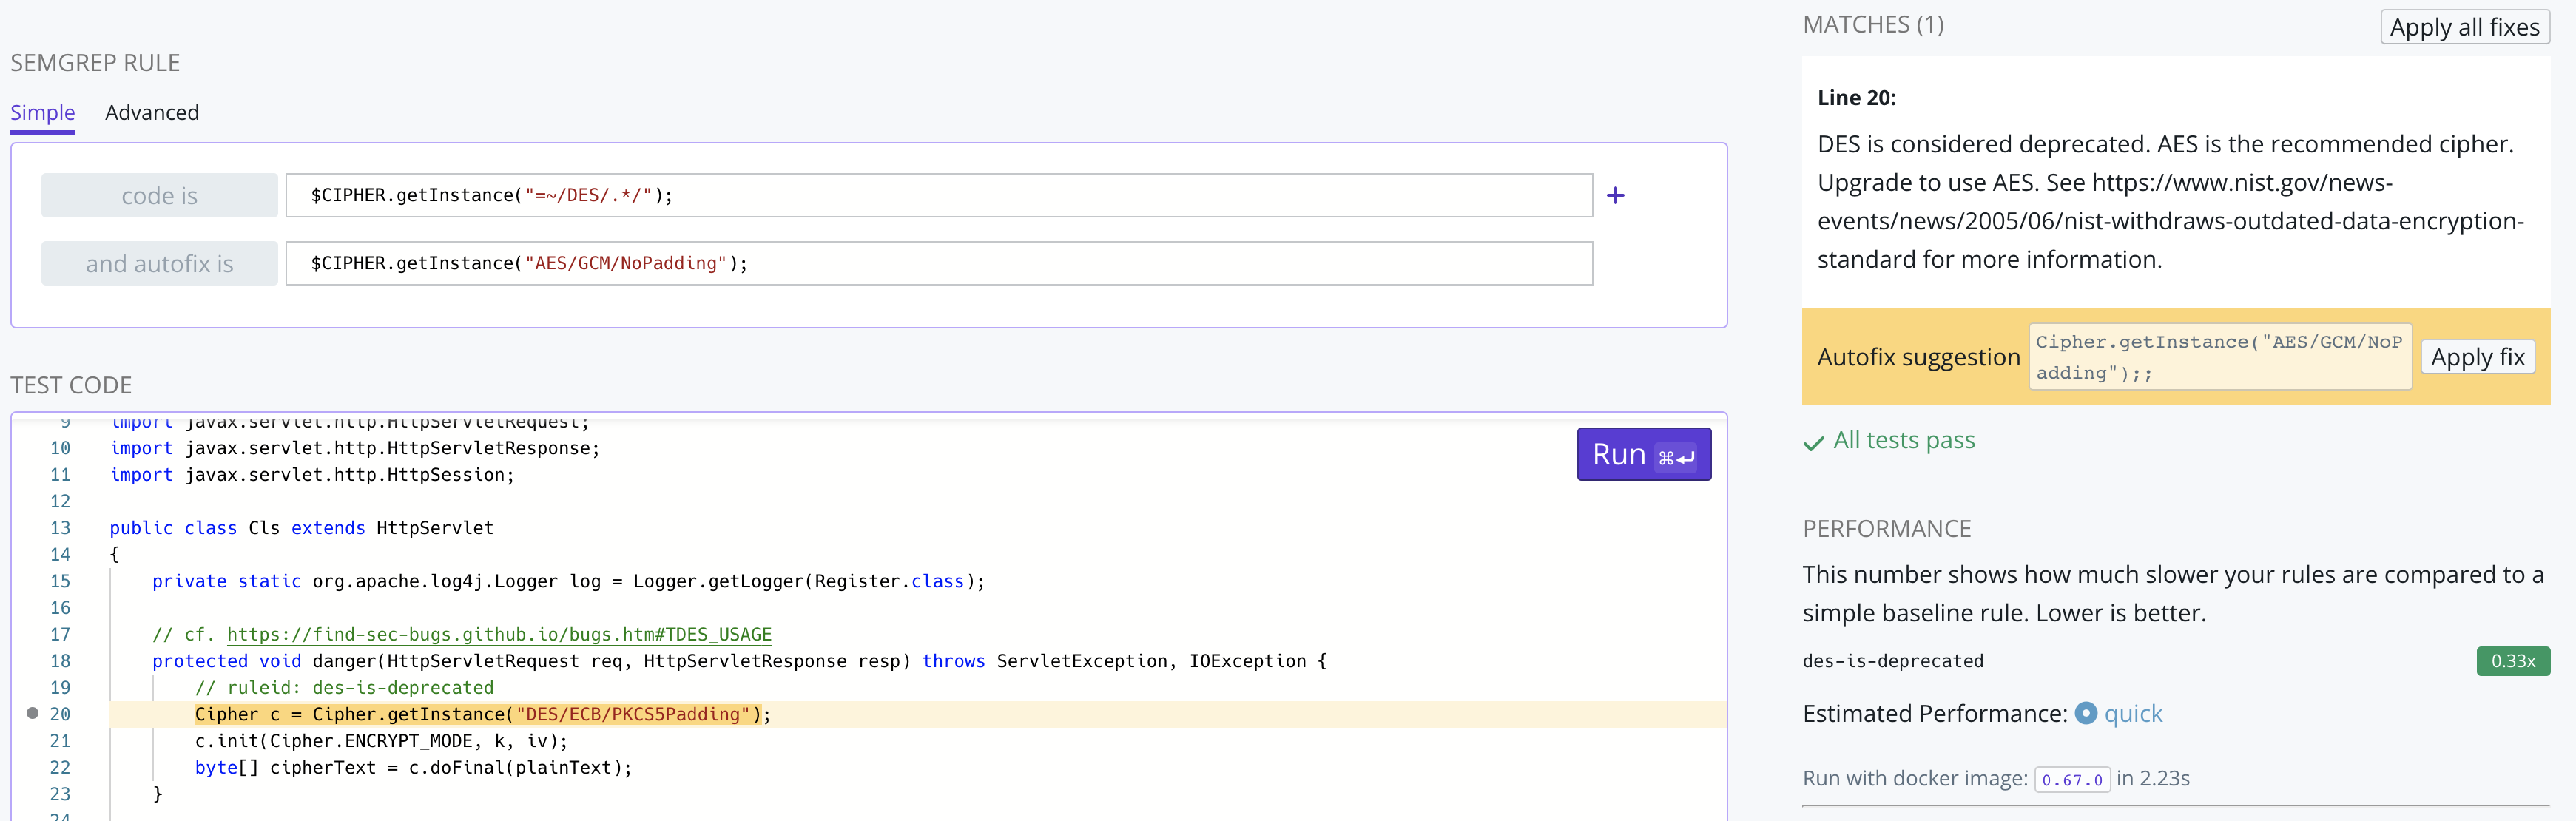
\includegraphics[width=\textwidth]{semgrep-editor.png}
  %\includegraphics[width=\textwidth,page=10]{04-tools/figures/figures2.pdf}
  \caption[Semgrep playground editor]{Semgrep's ``Simple" view in the Playground rule editor still requires use of the \gls{yaml} syntax.}
  \label{fig:semgrep-editor} 
\end{sidewaysfigure}

Semgrep also provides a few advanced features such as taint tracking which is similar to the concept of trusted input in Sensei.
To use taint tracking in a rule, sources and sinks need to be defined as well as optional sanitizers.
Since taint tracking requires a source to be specified, it functions differently to the trusted input of Sensei, where all input is untrusted by default.
Using metavariables it is possible to create a rule that prevents \glspl{efp} similarly to Sensei's trusted input. 
Listing~\ref{lst:metavariable} shows a rule to detect potential \gls{os} command injections, the analogous Sensei recipe is shown in Listing~\ref{lst:yamlrecipe}, but repeated here in Listing~\ref{lst:oscommand-sensei} for convenience.


\begin{minipage}[t]{0.9\linewidth}
\begin{lstlisting}[language={yaml},caption={Any commands passed on to the \texttt{exec} method that have not been retrieved through \texttt{getSafeCommand} will be marked.},label={lst:metavariable},xleftmargin=15pt]
rules:
- id: os-command
  patterns:
    - pattern: $RUNTIME.exec($COMMAND)
    - pattern-not-inside: |
        $COMMAND = getSafeCommand();
        ...
        $RUNTIME.exec($COMMAND);
  message: "Could lead to OS Command injection"
  languages: [java]
  severity: ERROR

\end{lstlisting}

\begin{lstlisting}[language={yaml},caption={Any input is untrusted by default except input retrieved through \texttt{getSafeCommand}. Untrusted input passed on to the \texttt{exec} methodcall will be marked.},label={lst:oscommand-sensei},xleftmargin=15pt]
search:
  methodcall:
    name: "exec"
    type: "java.lang.Runtime"
    args:
      1:
        type: "java.lang.String"
        containsUntrustedInput: true
        trustedSources:
        - methodcall:
            name: "getSafeCommand"
\end{lstlisting}
\end{minipage}
\section{Release and deploy}

High velocity of development and delivery is most easily achieved in \gls{saas} and other cloud computing delivery models.
It is easier to push frequent updates if there is only a single version of the application running, hosted centrally and managed by the software provider.
Furthermore, because the service provider has access to user data and behaviour, it is easier to collect feedback and make incremental improvements.
Finally, it is more economically viable to adapt to continuously changing requirements of customers, if the software is sold on a subscription basis.

\subsubsection{Infrastructure as code}
To keep pace with this high velocity of software development, new technology has been developed to automate infrastructure and deployment.
With \gls{iac}, the process of managing and provisioning data centers is done through machine-readable configuration files rather than hardware configurations and interactive tools~\cite{wittig2018amazon}.
Most frequently these configuration files are declarative, focusing on what the eventual target configuration should be, rather than describing the necessary changes to meet this configuration.
Two big components are required for automated infrastructure, those are application deployment and runtime orchestration.

\paragraph{Application deployment}
Modern software applications often consists of a variety of services, such as an \gls{api}, a web front-end, a back-end application, logging services, and services used for data analytics.
To ease the deployment, and to isolate services from each other, virtualization is used.
In early virtualization, a \gls{vmi} was created that contains the service's code and any requirements to run it, such as the \gls{os} and the dependencies.
A \gls{vmi} is a from of hardware virtualization, each is deployed as \textit{guests} on a \textit{host} machine, providing its own \gls{os} with its own kernel.
Because of this, \glspl{vm} can be deployed anywhere without requiring modifications.
This also has the added benefit of isolation between different services, so that each one has a fixed amount of \gls{cpu} processing power and memory.
However, they are large and take a lot of resources to store and run.

More modern technology moves from hardware virtualization to \gls{os}-level virtualization.
Here, the kernel of the host \gls{os} allows the existence of multiple isolated user space instances, called containers.
The most popular container technology today is Docker\footurl{https://www.docker.com/}.
With docker the application and its dependencies ara packaged in a virtual container that can run on any \gls{os}.
Docker containers are more lightweight, and a single server or \gls{vm} can run several containers simultaneously.
A docker container image is built by reading instructions from a Dockerfile\footurl{https://docs.docker.com/engine/reference/builder/}.
This file contains a selection of commands that a user could call on the command line interface to assemble the image.
An example of a Dockerfile is shown in Listing~\ref{lst:Dockerfile}.
The image is built from an ubuntu docker image. Then the contents from the \texttt{app} directory are copied to the image and the application is built using the make command. Finally the app is started.
Containers make it easy to control data and software components and make frequent updates such as security patches.

\begin{lstlisting}[language={Dockerfile},caption={Example of a Dockerfile to build and run a Python application.},label={lst:Dockerfile},xleftmargin=15pt]
# syntax=docker/dockerfile:1
FROM ubuntu:18.04
COPY . /app
RUN make /app
CMD python /app/app.py
\end{lstlisting}

Docker promotes the use of multi-container applications, where each service in the application is placed in its own container.
This is done through a docker-compose file, as shown in Listing~\ref{lst:dockercompose}.
This example, used during my research, sets up a mariaDB database and exposes it on port 3306. It also creates a web interface called Adminer, hosted on port 8080.

Placing separate services in their own containers like this, improves security, as containers, by default, run in isolation.
Each container can only access ports and files of other containers that are explicitly exposed by the other containers.

\begin{minipage}[t]{0.9\linewidth}
\begin{lstlisting}[language={YAML},caption={Example of a Dockerfile to build and run a Python application.},label={lst:dockercompose},xleftmargin=15pt]
version: '3.1'
services:
  maria:
    image: mariadb
    ports:
      - 3306:3306
    volumes:
      - mariadb:/var/lib/mysql
  web:
    image: adminer
    ports:
      - 8080:8080
volumes:
  mariadb:

\end{lstlisting}
\end{minipage}

Docker increases the level of security in comparison to running applications directly on the host.
It has features to more easily encrypt volumes, manage secrets, and encrypt communication between containers, all helping to avoid some of the top categories in the \gls{owasp} top 10.
But some misconfigurations can still downgrade the level of security and even introduce new vulnerabilities.
Many guides and training exist to help secure Dockerfiles and other container technology, including on the \gls{scw} portal, the \gls{owasp} website\footurl{https://cheatsheetseries.owasp.org/cheatsheets/Docker_Security_Cheat_Sheet.html}, and even \gls{nist}\footurl{https://csrc.nist.gov/publications/detail/nistir/8176/final}.
Some security tools, like Snyk, have adapted to scan for container misconfigurations, to detect, for example, use of containers with known vulnerabilities.

\paragraph{Runtime orchestration}
With runtime orchestration, the management of multiple physical servers is being abstracted as well.
An orchestration framework exposes a server cluster as if it were a single pool of resources, and allows the installation and management of containers across these servers from one centralized host.
Several runtime orchestration frameworks exist, with the most popular being Kubernetes (K8s), originally designed by Google and now maintained by the 
\gls{cncf}.
Runtime orchestration makes it easy to apply security practices such as network encryption, authentication, and management of application secrets\footurl{https://kubernetes.io/docs/concepts/security/overview/}. 

Kubernetes is designed to be highly customizable and developers must turn on certain features to make sure the resulting configuration is secure.
More information can be found on the \gls{owasp} website\footurl{https://cheatsheetseries.owasp.org/cheatsheets/Kubernetes_Security_Cheat_Sheet.html}.

\subsubsection{Policy as code}
With policy as code, isolation and decoupling is taken one step further.
A separate service is deployed that can be queried to make policy decisions.
One framework to run such a service is \gls{opa}, backed up be \gls{cncf}.

As an example, take a look at authorization decisions.
In a budgeting application, manager may be able to access the salary of anyone who reports to them.
To make such decisions, the management chain can be stored in the policy agent, an example is shown how this can be stored in \gls{opa} in Listing~\ref{lst:mgmt-chain}.

\begin{lstlisting}[language={json},caption={Management chain data example for use in OPA.},label={lst:mgmt-chain},xleftmargin=15pt]
{
    "management_chain": {
        "colin": [
            "pieter",
            "downey"
        ],
        "alex": [
            "gillis"
        ]
    }
}
\end{lstlisting}

It is then possible to define rules and execute queries based on this data.
In Listing~\ref{lst:opa-rule} rules are shown for the salary example.
Users are allowed to see their own salary and that of other users below them in the management chain.


\begin{minipage}[t]{0.9\linewidth}
\begin{lstlisting}[language={json},caption={OPA rules that define who has access to the salary of other users.},label={lst:opa-rule},xleftmargin=15pt]
default allow = false

allow {
    input.method = "GET"
    input.path = ["salary", id]
    input.user_id = id
}

allow {
    input.method = "GET"
    input.path = ["salary", id]
    managers = data.management_chain[id]
    input.user_id = managers[_]
}
\end{lstlisting}
\end{minipage}

The budgeting application can then make decisions by querying the \gls{opa} service as shown in Listing~\ref{lst:opa-query}.

\begin{minipage}[t]{0.9\linewidth}
\begin{lstlisting}[language={java},caption={Management chain data example for use in OPA.},label={lst:opa-query},xleftmargin=15pt]
> input := {"method": "GET", "path": ["salary", "colin"], "user_id": "gillis"}
> allow
false
\end{lstlisting}
\end{minipage}

Decoupling policy decisions like this has many advantages.
It provides a centralized overview of policies and avoids redundancy in implementations.
In another application, for example, employees are able to request absence and these requests can be authorized by their manager.
Instead of implementing these decisions again in the second application and possibly even storing the data multiple times, the \gls{opa} service can be reused by adding new rules.

Because of the declarative nature of the rules, they can be understood easily, causing reduced complexity and hence reduced chance for mistakes.
The policy agent can be used to overcome several vulnerabilities in \gls{owasp} top 10, such as authentication and authorization decisions, as well as some business logic flaws.

By using a policy as code service, logging of the policy decisions will also be done separately from application logs.
This can make it easier to monitor and detect abnormal usage of the application, partly mitigating the security problem of excessive logging in the application itself.

%\section*{List of stuff to look at}
%Check these sources: 
%https://owasp.org/www-community/Source\_Code\_Analysis\_Tools
%https://owasp.org/www-community/Vulnerability\_Scanning\_Tools
%https://kompar.tools/
%https://securecodewarrior.atlassian.net/wiki/spaces/CP/pages/993329838/Why+wouldn+t+you+use+X+instead
%https://securecodewarrior.atlassian.net/wiki/spaces/CP/pages/1103265877/Sensei+Competitive+Space
%
%Open Policy Agent (OPA)!!
%github copilot
%amazon guru
%\paragraph{Tricorder}
%\subsection{WhiteSource Cure}
%WhiteSource cure
%
%WhiteSource Cure looks interesting at a glance. But if you dig into it a bit, I think they’ve taken a few major short-cuts and odd decisions.
%They decide to not parameterize all inputs to a SQL query. This is bad because it shows to developers that it’s OK to not always parameterize all inputs.
%There’s some interesting comments in some of the fixes. If a setFeature call fails on a DocumentBuilderFactory, they are suggesting you should check for possible attack. That’s kind of FUD. That suggests no attack whatsoever.
%They are not detecting super obvious SQL injection issues right next to other fixes they are providing.
%Some of their suggestions handle things in a way that’s not exactly how I’d do it. For instance, their fix for path traversal needs 2 more changes by a developer to work without causing major issues. And it makes assumptions about the correct design that I don’t think are valid. You’re thus not fixing the issue at its root.
%https://securecodewarrior.slack.com/archives/C92HYQNVA/p1627890321009700
%
%\paragraph{ReshiftSecurity}
%TODO: %https://www.reshiftsecurity.com/product/ 
%- based on Spotbugs and (I think) the SpotBugs security plugin
%- does not play nice with spotbugs (removes ability to configure spotbugs preferences ) so I think they may not have amended Spotbugs code enough to make it an independent plugin
%- autofix functionality doesn't appear to be present in the IDE, I think that is through a CI integration
%- don't think you can create your own rules easily
%- not sure how good it is at identifying security issues, it did not pick up an SQL injection in my sample project
%```
%            Statement stm = dbConnection.createStatement();
%            ResultSet res = stm.executeQuery(
%                    "SELECT description from todos where status=" + status);
%```
%
%%%https://www.producthunt.com/posts/reshift-security
%\paragraph{Semmle}
%  %https://www.theregister.co.uk/2020/05/06/github\_releases\_codescanning\_tool/
%  Semmle is cool stuff. But:
%It’s not a developer-focused tool per say. It’s complex, and requires appsec to write rules
%It’s not in your IDE
%It is very focused on “Is this exploitable?“, which means it’s not useful for enforcing code best practices
%It doesn’t give you quick-fixes
%It doesn’t give you contextual education
%Hence, it doesn’t close the loop to help prevent them from reoccurring
%
%\paragraph{CodeInspector}
%%%https://www.code-inspector.com/
%\paragraph{Semgrep}
%%https://r2c.dev/blog/2020/be-careful-what-you-request-for-django-method/ 
%%https://r2c.dev/blog/2020/hardcoded-secrets-unverified-tokens-and-other-common-jwt-mistakes/
%\paragraph{Pluralsight}
%%https://help.pluralsight.com/help/vs-code-extension
%
%\paragraph{RuleGuard}
%
%\paragraph{Explore.dev}
%%https://explore.dev/
%
%\paragraph{Deepcode}
%(Matias:)
%deepcode.ai
%Deepcode is a University project spin off (Spun of in 2016). It’s focus was on quality code, not security in specific.
%Focus on:
%* Accuracy
%* Speed
%* For developers
%When demoing, main focus went to the IDE plugin (Can also work in Pull request and in CD/CD). Demo was very slick. it shows errors and warnings, and it shows other places in the code where a developer made that change before, essentially they went through the entire history of checkins and make rules out of that (not really rules, it is in their AI/ML module). So it is not only finding, it does have a focus on real fixes, potentially in line with the code base, stuff that can actually work.
%AI/ML component is very interesting. AI/ML instead of rules based is very interesting. If this works, if they can pull that off, it is a good approach to get rid of manual effort and still be custom to the code (but that is not the focus, so this is not happening right now). It diminishes the number of researchers they have to have on staff to create rules. It reduces the time to value for customers using the solution.
%Compared to Semmle: Seems to have a lot of similarities. Started as a tool focused on quality, not specifically security. Was a university project first which was incubated, so not really a focus on making this work at scale. (Great for a demo, great in theory, great on a small code base, but what about the real world). However, from what they have shown, it looks better/easier/slicker/more mature than Semmle.
%If the demo works in practice on large codebases, then I think it will be a significant challenger for the established SAST solutions.
%I think there is an opportunity for SCW to be in there and educate the developer. The examples in the demo were simplistic (hardcoded passwords) so there was no need for training, but I can see a role for the SCW training platform with what I’ve seen
%Sensei, that becomes more interesting, but there are advantages and disadvantages. Sensei is still real-time, Snyk Code is when pressing a button, and in a different window. Sensei has a quick fix, Snyk does not have one. Sensei is more tailored to the code, Snyk is not. But then there are undeniable advantages of their approach. The ML/AI instead of rules should be better in terms of configuration, rules support, … if and only if this AI/ML thing work. And that AI/ML thing may show quicker value than Sensei, as the upfront work is less on Snyk code. Sensei feels more enterprise than Snyk code tbh, I don’t see them doing what we do at NetSuite, that AI/ML is too free form and can propose whatever.
%
%(Brysen:)
%I just watched the demo videos on their youtube channel.
%Sending your code to their servers is an annoying thing.
%The way they provide a “fix” is done by showing you examples of open source repos where this issue should have been fixed, but in their example it doesn’t even show the same code as the found vulnerability so effectively the user still needs to plow through the suggested changes and determine if they are right in which they still need a good too strong security knowledge.
%
%Specifically to Sensei, one thing we have to copy is showing an example. So the suggestion they make is together with an example of another place in the code where this is also the case (or where that same change was executed). That looked really cool. I think in Sensei that would work even better, because we should do that in the code base itself, and not on some random other open source project... My 2 cents
%
%\subsubsection{Fortify}
%Micro Focus Fortify is an ecosystem that embeds application security testing into all stages of the development tool chain. Some of the most comparable tools to Sensei in their ecosystem are Fortify Static Code Analyzer (FSCA), Fortify on Demand (FOD), and Fortify Security Assistant (FSA). 
%
%As the name suggests, FSCA~\cite{fsca} performs static code analysis on the source code. It can be built in CI/CD tools and has support for 25 programming languages including Java and C\#. Scanning takes several minutes and the results can be shown in a web interface or in integrations with many bug tracking systems, ticketing systems, and code repositories. Fortify recommends using their rule sets that cover over 1000 vulnerability categories and more than one million APIs. Creating new rules can be done in their custom XML format in any text editor~\cite{fsca-curstom-rules}. Doing so requires reading extensive documentation and learning the proper syntax. They do not provide a rule editor, instead the rule writer can use any preferred text editor. FOD~\cite{fod} provides similar features to FSCA but through a web portal, Micro Focus calls this Application Security as a Service. 
%
%FSA~\cite{fsa} is a plugin for the IDE, currently available for Eclipse and Visual Studio. It allows security scans in the IDE, where the rule set is tuned such that the longest analyses are disabled by default. The scan can take several minutes during which the developer cannot make any code changes. This is still quite long compared to the real-time results of Sensei and might inhibit developers from requesting scans frequently during development. 
%
%%\changed{As already discussed in Section \ref{sec:evaluation} this demonstrates the trade-off for early detection: a more light-weight version of the analyses is performed in the IDE to guarantee the developers' usability, which means that not all potential issues can be detected at this stage.}
%
%Besides the FSA, Fortify offers two more IDE plugins. The FOD plugin is available for Eclipse, Visual Studio, and IntelliJ. It allows the developer to request static assessments from FOD and download the results. A similar plugin is available for FSCA on all three IDEs. 
%
%FOD allows scan results to be evaluated against custom security policies in order to hide reports of certain vulnerability types. During installation of the FSA in the IDE, a link to a remote Rulepack Update Server is required, this allows the tool to download the necessary rule information to perform scans. It is also possible to use a local copy of the rules when no network connection is available. The FSA also allows enabling and disabling each individual rule in the UI. 
%
%Each tool provides detailed descriptions on vulnerabilities, which focus on explaining the vulnerabilities in detail, in part by providing examples of insecure code. In a second tab, FOD provides a description and code examples to resolve the vulnerability. All tools provide links to reference material and to recommended solutions. FOD also provides links to Secure Code Warrior to provide training on a specific vulnerability. The information provided is very similar to the different descriptions of Sensei, but the focus is more on explaining the vulnerability first instead of the solution.
%
%Both FSCA and FOD provide a management dashboard in which the security status (failed or passed security policy) of multiple applications can be seen. The dashboard of FOD provides more detailed information where it is possible to track the amount of issues over time for each severity. It also provides an insight in the vulnerability categories of most prevalent issues. FOD can track the amount of newly introduced problems in each scan. This makes it possible to evaluate the developers' skills over time, on top of tracking the application state. However, in contrast to Sensei, no clear distinction is made between problems detected by new rules and problems detected in newly developed code.
%
%\subsubsection{Tricorder}
%
%
%\subsubsection{SpotBugs}
%
%
%\subsubsection{SecureAssist}
%SecureAssist~\cite{secureassist} is an IDE plugin targeting the discovery of security bugs in code. It is available for eclipse, intelliJ, VisualStudio, RAD, and Spring Tool Suite~\cite{sastinide}. Its scans are not in the IDE but on the enterprise portal. The results are sent back to the IDE once completed. This allows scanning without preventing the developer from continuing his work, which contrasts with the Fortify Security Assistant, that prevents developers from changing the code during a scan. Remediation is provided in the form of descriptions that explain the attack and provide some code examples but the tool does not provide quick fixes~\cite{secureassistide}. 
%
%Rule packs are distributed as JAR files and the tool provides a Rulepack Configurator similar to Sensei's cookbook Manager.
%
%\subsubsection{Veracode}
%Veracode offers two tools. The Veracode Static Analysis (VSA) is a SaaS platform that is similar to Fortify on Demand~\cite{veracode}. Veracode Greenlight (VG) is an IDE plugin, similar to Fortify Security Asisstant.
%
%VSA performs static analysis scans on compiled bytecode of web applications in 23 programming languages. Because it does not need access to the source code it can also analyse frameworks and libraries used in the project. VSA provides integrations with popular ticketing systems, CI/CD tools and three IDEs: IntelliJ, Visual Studio, and Eclipse. All these integrations offer the possibility to start scans and download the results. Veracode focuses heavily on not only detecting vulnerabilities but also guiding remediation. To that extent, they provide detailed instructions and videos. There is even the possibility to schedule a one-on-one conference call with a consultation expert. This expert can help the developer determine whether an issue is a false positive or what the best remediation is for a detected vulnerability. Scheduling such a consultation will usually take about three days. Veracode does not encourage or provide help to share the knowledge that is gathered by the developer during such a consultation session with their peers. 
%
%The company claims most scans finish in under an hour. This means the feedback cycle is rather long compared to the other tools. Since the scans are performed on binaries, they are not able to provide quickfixes as Sensei does, which is unfortunate for a solution otherwise very focused on remediation.
%
%Veracode promotes a low false positive rate of 5\% and hence discourages rule customization. Rule customization would also be much harder, since VSA analyzes compiled bytecode, not source code. VSA does not allow to disable rules or issues individually, but lets companies define a custom security policy for their application. Setting a policy configures the conditions used to evaluate results of  a scan, and helps decide if the build should break or be accepted. In these policies it is possible to add rules that disable certain CWE entries, category of flaws, or severity of flaws. Veracode offers Program Management Support, where a Program Manager will help define these policies, and gradually increase their requirements. This helps guarantee developer usability during roll-out. Developers will first be encouraged to resolve the most severe issues. In later stages when a tighter policy is set, they are exposed to additional issues. Although a new policy does not provide as granular control as a new rule in Sensei, this feature and roll-out procedure closely resemble the best practices described in Section \ref{sec:rollout}.
%
%VSA offers a dashboard to track scan results over time. This displays the number of flaws per scan, tracks which ones are new, and organises the existing flaws into severity categories.
%
%VG is an IDE plugin for Eclipse, IntelliJ, and Visual Studio. It is a light-weight version of VSA that is scanned locally. Since the scans are performed on bytecode, it requires a successful build. VG can be configured to scan automatically by using the Automatic Build option in the IDE. Scans are not real-time like Sensei but take around 3 seconds, after which the results are not shown in the IDE editor, but in a separate pane. Double clicking an issue in this pane will open the editor at the relevant location in code. Like VSA, VG is unable to provide quickfixes, but provides a lot of detailed information to the developer.
%
%\subsubsection{Checkmarx}
%Checkmarx Static Application Security Testing (CxSAST)~\cite{cxsast} is a static analysis tool that perfoms source code scans. It has support for over 25 coding and scripting languages, including Java, C\#, and python. Similar to Fortify and Veracode, CxSAST has IDE plugins for Eclipse, Visual Studio, and IntelliJ. Again, and still in contrast to Sensei, these plugins do not perform any local scans but instead allow uploading the source code to CxSAST. They provide an interactive way to view the scan results by marking the relevant code in the IDE editor. 
%
%Checkmarx claims flexible rules lead to higher accuracy, and have a very extensive Query Language (CxQL)~\cite{cxaudit} to create and adapt rules.  Managing queries is done in the CxAudit tool, this tool allows enabling and disabling individual queries. Here, new queries can also be added in a Query Source Pane. It is possible to export a set of queries from this tool to use in different applications. The source pane however provides little help to write and especially debug new rules. Since the rule-writing tool is independent from the scanning tool and the IDE, it requires long iterations to optimize rules compared to the instant feedback in the Sensei rule editor where the results of rules are updated live. Vulnerabilities marked in the scan results have a category but no descriptions are provided. This means that little help is provided compared to the remediation suggestions and quickfixes of Sensei. More details about the control flow leading to the vulnerability are clearly marked in the IDE plugins and can help an experienced developer find the best place in source code to resolve the problem. A similar feature could be developed for Sensei's concept of trusted input, but it was decide to omit this to avoid unnecessary clutter in the IDE.
%
%Checkmarx does provide an integration between CxSAST and its training service CxCodebashing. This way developers can learn about the vulnerability and how to fix it in an interactive way. This integration is similar to the integration between Secure Code Warrior and Fortify on Demand, as well as the training links in the full coding guideline description of Sensei.
%
%\subsubsection{Aside}
%The OWASP ASIDE/ESIDE~\cite{aside} project consist of two branches, the ASIDE branch that focuses on detecting software vulnerabilities and helping developer write secure code, and the ESIDE branch that focuses on helping students in acquiring secure programming knowledge and practices.
%
%Application Security IDE (\emph{ASIDE}) performs fast scans of the code in Eclipse, but unlike Sensei the scans need to be started manually. Besides detecting vulnerabilities they also provide quick fixes for some issues. The quick fixes require the developers to choose from a list of options, which could overwhelm them. In previous research a large number of false positives were detected~\cite{xie2011aside}, however, most of these are what is considered protection for future use in this paper. They are cases where best practices should be applied even if their violation is not yet exploitable at this point in development. They also mark variables in the code that are tainted, this could be compared to Sensei's concept of untrusted input. Untrusted input in Sensei is not currently marked to avoid unnecessary clutter. 
%
%The goal of ESIDE~\cite{eside,whitney2018embedding} is to provide information and training at all times during the education. Its rules can not be configured and the tool does not provide quickfixes. However they provide explanation in external web pages linked from Eclipse. Their information is similar to our full coding guidelines where information on APIs and a correct code example is provided. 
%
%
%
%
%
%
%